\documentclass{beamer}
\usetheme{Boadilla}
\usecolortheme{default}
\usepackage[utf8]{inputenc}
\usepackage{amsmath}
\usepackage{amsfonts}
\usepackage{amssymb}
\usepackage{amsthm}
\usepackage{array}
\usepackage{float}
\usepackage{listings}
\usepackage{color}
\usepackage{caption}
\usepackage{multirow}
\usepackage{xcolor}
\usepackage{colortbl}
\usepackage{caption}
\usepackage{subcaption}
\usepackage{multimedia}
\usepackage{tikz}
\usepackage{varwidth}
\usepackage[absolute,overlay]{textpos}
\usetikzlibrary{shapes.misc,shadows}
\usetikzlibrary{quotes,positioning,arrows,decorations.markings}
\usetikzlibrary{positioning,backgrounds} 
\usepackage[cache=true,section]{minted}
\usepackage[algosection,linesnumbered]{algorithm2e}
\usepackage{glossaries}
\usemintedstyle{default}

\def\HiLi{\leavevmode\rlap{\hbox to \hsize{\color{yellow!50}\leaders\hrule height .8\baselineskip depth .5ex\hfill}}}
\definecolor{androidgreen}{rgb}{0.64,0.78,0.22}
\definecolor{titaniumyellow}{rgb}{0.93,0.9,0.0}
\definecolor{light}{rgb}{0.5, 0.5, 0.5}
\newtheorem{complexity}{Complexity}

\makeatletter
\long\def\beamer@author[#1]#2{%
  \def\insertauthor{\def\inst{\beamer@insttitle}\def\and{\beamer@andtitle}%
  \begin{tabular}{rl}#2\end{tabular}}%
  \def\beamer@shortauthor{#1}%
  \ifbeamer@autopdfinfo%
    \def\beamer@andstripped{}%
    \beamer@stripands#1 \and\relax
    {\let\inst=\@gobble\let\thanks=\@gobble\def\and{, }\hypersetup{pdfauthor={\beamer@andstripped}}}
  \fi%
}
\makeatother

\setbeamercolor{block title}{bg=blue!10, fg=black}
\setbeamercolor{block body}{bg=white!25}

\tikzset{
    max width/.style args={#1}{
        execute at begin node={\begin{varwidth}{#1}},
        execute at end node={\end{varwidth}}
    }
}

\newcommand{\itemcheck}{\item[\checkmark]}

\title[Incrementally Enumerating BT in BG]{An Algorithm for incrementally Enumerating Bitriangles in large Bipartite Networks}
\subtitle{Master Thesis\vspace{-0.5cm}}
\author[Juan Pablo Royo Sales (Master Thesis)]{\vspace{-0.5cm}Juan Pablo Royo Sales}
\institute[]{%
  {\small Facultat d’Informàtica de Barcelona (FIB)}\\
  {\small Universitat Politècnica de Catalunya (UPC) – BarcelonaTech}\\
  \vspace{0.2cm}
  Master in Innovation and Research in Informatics\\ 
  Advance Computing\\
  \vspace{0.2cm}
  \tiny{%
  Supervisors: Edelmira Pasarella, Computer Science Department\\
  Maria-Esther Vidal, Leibniz Information Centre for Science and Technology-TIB, and L3S Centre at the Leibniz University of Hannover\\
  Cristina Zoltan, Computer Science Department
  }
}

\date[October 29, 2021]{October 29, 2021}
  
\titlegraphic{%
  \begin{tikzpicture}[overlay,remember picture]
    \node[left=3.5cm] at (current page.30){
      
\includegraphics[height=1.5cm]{upc_logo}
    };
  \end{tikzpicture}
}

\usetikzlibrary{external,quotes,positioning,calc,arrows,decorations.markings,positioning,fit,shapes.misc,shadows}
\tikzstyle{bag} = [align=center]

\usemintedstyle{default}
\newminted{haskell}{frame=lines,framerule=2pt}
\newminted{R}{frame=lines,framerule=2pt}

\graphicspath{{./images/}}

\newcommand{\dw}{\mathbb{DW}}
\newcommand{\aw}{\mathbb{AW}}
\newcommand{\bt}{\mathbb{BT}}
\newcommand{\bti}{BT_{(l_1, l_2,l_3)}^{(u_1, u_2, u_3)}}
\newcommand{\at}{\mathbb{AT}}
\newcommand{\dwi}{\mathsf{dw}}
\newcommand{\ati}{\mathsf{at}}
\newcommand{\btii}{\mathsf{bt}}
\newcommand{\st}{ST}
\newcommand{\sw}{\mathtt{spawn}}
\newcommand{\fd}{\mathtt{killFilter}}
\newcommand{\fid}{\mathtt{filterIsDead}}
\newcommand{\us}{\mathtt{updateState}}
\newcommand{\gs}{\mathtt{getState}}
\newcommand{\p}{\mathtt{push}}
\newcommand{\mt}{\mathtt{matchQ}}
\newcommand{\io}{\mathtt{indexOf}}
\newcommand{\la}{\left\langle}
\newcommand{\ra}{\right\rangle}
\newcommand{\DP}{\mathsf{DP}}
\newcommand{\dpbt}{\mathsf{DP_{BT}}}
\newcommand{\ibt}{\mathsf{Sr_{BT}}}
\newcommand{\obt}{\mathsf{Sk_{BT}}}
\newcommand{\fbt}{\mathsf{F_{BT}}} 
\newcommand{\gbt}{\mathsf{G_{BT}}}
\newcommand{\dpwcc}{\mathsf{DP_{WCC}}}
\newcommand{\iwcc}{\mathsf{Sr}}
\newcommand{\iwc}{\mathsf{Sr_{WCC}}}
\newcommand{\owcc}{\mathsf{Sk}}
\newcommand{\owc}{\mathsf{Sk_{WCC}}}
\newcommand{\fwcc}{\mathsf{F}} 
\newcommand{\fwc}{\mathsf{F_{WCC}}} 
\newcommand{\gwcc}{\mathsf{G}}
\newcommand{\gwc}{\mathsf{G_{WCC}}}
\newcommand{\ice}{\mathsf{IC_E}}
\newcommand{\csofv}{\mathsf{IC_{set(V)}}}
\newcommand{\sgen}{\mathsf{S_G}}
\newcommand{\sfilter}{\mathsf{S_F}}
\newcommand{\sinp}{\mathsf{S_I}}
\newcommand{\sout}{\mathsf{S_O}}
\newcommand{\istream}{\mathsf{D}}
\newcommand{\wccout}{\mathsf{R}}
\newcommand{\fmem}{\mathsf{M_F}}
\newcommand{\eof}{\mathsf{eof}}
\newcommand{\Act}{\mathsf{actor_1}}
\newcommand{\Actt}{\mathsf{actor_2}}
\newcommand{\gdsl}{G_{dsl}}
\newcommand{\aaa}{\mathsf{actor_1}}
\newcommand{\ab}{\mathsf{actor_2}}
\newcommand{\ac}{\mathsf{actor_3}}
\newcommand{\ad}{\mathsf{actor_4}}

\renewcommand*{\listlistingname}{List of Source Code}

\renewcommand\listingscaption{Source Code}
\providecommand*{\listingautorefname}{Source Code}

\DeclareMathOperator*{\argmax}{arg\,max}
\DeclareMathOperator*{\argmin}{arg\,min}

\newacronym{bt}{BT}{Bitriangle}
\newacronym{bg}{BG}{Bipartite Graph}
\newacronym{iebt}{IEBT}{Algorithm for Incrementally Enumerating Bitriangles in Large Bipartite Network}
\newacronym{ug}{UG}{Unipartite Graph}
\newacronym{dp}{DPP}{Dynamic Pipeline Paradigm}
\newacronym{dpf}{DPF}{Dynamic Pipeline Framework}
\newacronym{wg}{WG}{Wedge}
\newacronym{awg}{AW}{Aggregated Wedge}
\newacronym{dwg}{DW}{Double-wedge}
\newacronym{adwg}{ADW}{Aggregated double-wedge}
\newacronym{abt}{ABT}{Aggregated Bitriangle}
\newacronym{qo}{QO}{Query Operator}
\newacronym{awgc}{AW-BT}{Aggregated wedge BT-Connector}
\newacronym{dpfh}{DPF-Haskell}{Haskell Dynamic Pipeline Framework}
\newacronym{ds}{DS}{Data Streaming}
\newacronym{dap}{DAP}{Data Parallelism}
\newacronym{pip}{PP}{Pipeline Parallelism}
\newacronym{mr}{MR}{MapReduce}
\newacronym{hack}{Hackage}{The Haskell Package Repository}
\newacronym{dpbt}{DP-BT-Haskell}{$DP_{BT}$ in Haskell}
\newacronym{dpwcc}{DP-WCC-Haskell}{$DP_{WCC}$ in Haskell}
\newacronym{wcc}{WCC}{Weak Connected Components}
\newacronym{cfg}{CFG}{Context-Free Grammar}
\newacronym{hs}{Haskell}{Haskell Programming Language}
\newacronym{dbpedia}{Dbpedia}{Dbpedia Network}
\newacronym{stm}{STM}{Software Transactional Memory}
\newacronym{os}{OS}{Operative System}
\newacronym{dt}{\texttt{dief$@$t}}{Diefficiency Metric \texttt{dief$@$t}}
\newacronym{dk}{\texttt{dief$@$k}}{Diefficiency Metric \texttt{dief$@$k}}
\newacronym{dtkp}{\texttt{diefpy}}{\texttt{diefpy} Tool}
\newacronym{tfft}{TFFT}{Time for the first tuple}
\newacronym{et}{ET}{Execution Time}
\newacronym{comp}{Comp}{Completeness}
\newacronym{tt}{T}{Throughput}
\newacronym{snap}{SNAP}{Stanford Network Data Set Collection}
\newacronym{ghc}{GHC}{Glasgow Haskell Compiler}
\newacronym{dsl}{DSL}{Domain-specific Language}
\newacronym{edsl}{EDSL}{Embedded Domain-specific Language}
\newacronym{idl}{IDL}{Interpreter of DSL}
\newacronym{rs}{RS}{Runtime System}
\newacronym{mut}{MUT}{Mutator}
\newacronym{gc}{GC}{Garbage Collection}

\glsdisablehyper

\newtheorem{hyp}{Hypothesis}

\newcommand{\inputtikz}[1]{%
  \tikzsetnextfilename{#1}%
  \input{tikz/#1.tikz}
}

\makeatletter
\pgfdeclareshape{datastore}{
  \inheritsavedanchors[from=rectangle]
  \inheritanchorborder[from=rectangle]
  \inheritanchor[from=rectangle]{center}
  \inheritanchor[from=rectangle]{base}
  \inheritanchor[from=rectangle]{north}
  \inheritanchor[from=rectangle]{north east}
  \inheritanchor[from=rectangle]{east}
  \inheritanchor[from=rectangle]{south east}
  \inheritanchor[from=rectangle]{south}
  \inheritanchor[from=rectangle]{south west}
  \inheritanchor[from=rectangle]{west}
  \inheritanchor[from=rectangle]{north west}
  \backgroundpath{
    %  store lower right in xa/ya and upper right in xb/yb
    \southwest \pgf@xa=\pgf@x \pgf@ya=\pgf@y
    \northeast \pgf@xb=\pgf@x \pgf@yb=\pgf@y
    \pgfpathmoveto{\pgfpoint{\pgf@xa}{\pgf@ya}}
    \pgfpathlineto{\pgfpoint{\pgf@xb}{\pgf@ya}}
    \pgfpathmoveto{\pgfpoint{\pgf@xa}{\pgf@yb}}
    \pgfpathlineto{\pgfpoint{\pgf@xb}{\pgf@yb}}
 }
}
\makeatother

\tikzset{square arrow/.style={to path={-- ++(0,-0.5) |- (\tikztotarget)}}}
\tikzset{source/.style={shape=rectangle, minimum size=8mm}}
\tikzset{ionode/.style={shape=rectangle, draw=blue!50, fill=blue!5, very thick, minimum size=8mm, drop shadow={opacity=.5,shadow xshift=0pt}}}
\tikzset{ionode/.style={shape= rectangle, draw=blue!50, fill=blue!5, very thick, minimum size=8mm,drop shadow={opacity=.5,shadow xshift=0pt}}}
\tikzset{gennode/.style={shape= rectangle, draw=gray!50, fill=gray!5, very thick, minimum size=8mm, drop shadow={opacity=.5,shadow xshift=0pt}}}
\tikzset{filternode/.style={shape=rectangle, draw=cyan!50, fill=white, very thick, minimum size=8mm,drop shadow={opacity=.5,shadow xshift=0pt}}}
\tikzset{paramnode/.style={shape=rectangle, draw=cyan!50, fill=white, very thick, minimum size=8mm, 
drop shadow={opacity=.5,shadow xshift=0pt}}}
\tikzset{edge/.style = {->,> = latex}}
\tikzstyle{ioedge} = [thick, decoration={markings,mark=at position
   1 with {\arrow[semithick]{open triangle 60}}},
   double distance=1.4pt, shorten >= 5.5pt,
   preaction = {decorate},
   postaction = {draw,line width=1.4pt, white,shorten >= 4.5pt}]
\tikzset{indata/.style={draw,very thick, dotted,shape=datastore,inner sep=.3cm}}
\tikzset{outdata/.style={draw,very thick,shape=datastore,inner sep=.3cm}}




\usetikzlibrary{external,quotes,positioning,calc,arrows,decorations.markings,positioning,fit,shapes.misc,shadows}

\tikzexternalize[shell escape=-shell-escape,mode=graphics if exists,prefix=images/]


\begin{document}

  \begin{frame}
    \vspace{1.3cm}
    \titlepage
  \end{frame}

  \begin{frame}{Agenda}
    \tableofcontents[hidesubsections]
  \end{frame}
  
  \begin{frame}{Agenda}
    \section{Introduction}
    \tableofcontents[currentsection,hideothersubsections]
  \end{frame}

  \subsection{Goal}
  \begin{frame}[fragile]{Goal}
  \begin{center}
    Provide an Algorithm for Incrementally Enumarting Bitriangles in large Bipartite Networks using \textbf{Dynamic Pipeline Paradigm}
  \end{center}    
\end{frame}

\begin{frame}[fragile]{Goal}
  \begin{center}
    {\color{light}Provide an Algorithm for Incrementally Enumarting Bitriangles in large} \underline{{\color{red}\textbf{Bipartite Networks}}} {\color{light}{using \textbf{Dynamic Pipeline Paradigm}}}
  \end{center}    
  \begin{figure}
    \centering
    \resizebox{0.7\textwidth}{!}{\inputtikz{bipartite}}
  \end{figure}
\end{frame}

\begin{frame}[fragile]{Goal}
  \begin{center}
    {\color{light}Provide an Algorithm for Incrementally Enumarting} \underline{{\color{red}\textbf{Bitriangles}}} {\color{light}{in large Bipartite Networks using \textbf{Dynamic Pipeline Paradigm}}}
  \end{center}    
  \begin{figure}
    \centering
    \resizebox{0.7\textwidth}{!}{\inputtikz{bitriangle}}
  \end{figure}
\end{frame}



  \subsection{Motivation}
  % \begin{frame}[fragile]{Motivation}
%   \begin{center}
%     Provide an Algorithm for Incrementally Enumerating Bitriangles in large Bipartite Networks using \textbf{Dynamic Pipeline Paradigm}
%   \end{center}    
%   \vspace{0.5cm}
%   \begin{center}
%   \huge\emph{Why?}
%   \end{center}
% \end{frame}

\begin{frame}[fragile]{Motivation}
  % \begin{center}
  %   Provide an Algorithm for Incrementally Enumerating Bitriangles in large Bipartite Networks using \textbf{Dynamic Pipeline Paradigm}
  % \end{center}    
  \begin{itemize}
    \item \textbf{Bipartite Graphs} (BG) \underline{\color{red}models} interesting \underline{\color{red}relations} between \underline{\color{red}different set of objects}: i.e. \emph{diseasome bipartite networks, drugs-side effects networks, subscribers-TV show network, etc.}
  \end{itemize}
\end{frame}

\begin{frame}[fragile]{Motivation}
    \begin{itemize}
      \setlength\itemsep{2em}
      \item {\color{light}\textbf{Bipartite Graphs} (BG) models interesting relations between different set of objects: i.e. \emph{diseasome bipartite networks, drugs-side effects networks, subscribers-TV show network, etc.}}
      \item \textbf{Metrics} for analyzing BG \underline{\color{red}same as Unipartite Graphs}: \emph{clustering coefficient, communities, social analysis}.
    \end{itemize}
\end{frame}

\begin{frame}[fragile]{Motivation}
    \begin{itemize}
      \setlength\itemsep{2em}
      \item {\color{light}\textbf{Bipartite Graphs} (BG) models interesting relations between different set of objects: i.e. \emph{diseasome bipartite networks, drugs-side effects networks, subscribers-TV show network, etc.}}
      \item {\color{light}\textbf{Metrics} for analyzing BG same as Unipartite Graphs: \emph{clustering coefficient, communities, social analysis}.}
      \item \textbf{Projection method} distorts properties of original BG: i.e. link prediction.
    \end{itemize}
\end{frame}

\begin{frame}[fragile]{Motivation}
  \begin{itemize}
    \setlength\itemsep{1.5em}
    % \item {\color{light}Bipartite Graphs (BG) \textbf{models} interesting relations between \textbf{different set of objects}: i.e. \emph{diseasome bipartite networks, drugs-side effects networks, subscribers-TV show network, etc.}}
    % \item {\color{light}\textbf{Metrics} for \textbf{analyzing} BG same as Unipartite Graphs: \emph{clustering coefficient, communities, social analysis}.}
    % \item {\color{light}\textbf{Projection method} distorts properties of original BG: i.e. link prediction.}
    \item \textbf{Bitriangles} as the \underline{\color{red}small unit of cohesion} in BG. \textbf{Bitriangles counting} to compute \underline{\color{red}BG metrics} -- \emph{clustering coefficient, communities, social analysis} --.
  \end{itemize}
\end{frame}

\begin{frame}[fragile]{Motivation}
  \begin{itemize}
    \setlength\itemsep{1.5em}
    % \item {\color{light}Bipartite Graphs (BG) \textbf{models} interesting relations between \textbf{different set of objects}: i.e. \emph{diseasome bipartite networks, drugs-side effects networks, subscribers-TV show network, etc.}}
    % \item {\color{light}\textbf{Metrics} for \textbf{analyzing} BG same as Unipartite Graphs: \emph{clustering coefficient, communities, social analysis}.}
    % \item {\color{light}\textbf{Projection method} distorts properties of original BG: i.e. link prediction.}
    \item {\color{light}\textbf{Bitriangles} as the small unit of cohesion in BG. \textbf{Bitriangles counting} to compute BG metrics -- \emph{clustering coefficient, communities, social analysis} --.}
    \item Counting is \textbf{not enough}. Knowing \underline{\color{red}structural components of bitriangles} is needed: i.e.: \emph{what gene is involve in two or more diseases in diseasome networks}.
  \end{itemize}
\end{frame}

\begin{frame}[fragile]{Motivation}
    \begin{itemize}
      \setlength\itemsep{1.5em}
      % \item {\color{light}Bipartite Graphs (BG) \textbf{models} interesting relations between \textbf{different set of objects}: i.e. \emph{diseasome bipartite networks, drugs-side effects networks, subscribers-TV show network, etc.}}
      % \item {\color{light}\textbf{Metrics} for \textbf{analyzing} BG same as Unipartite Graphs: \emph{clustering coefficient, communities, social analysis}.}
      % \item {\color{light}\textbf{Projection method} distorts properties of original BG: i.e. link prediction.}
      \item {\color{light}\textbf{Bitriangles} as the small unit of cohesion in BG. \textbf{Bitriangles counting} to compute BG metrics -- \emph{clustering coefficient, communities, social analysis} --.}
      \item {\color{light}Counting is \textbf{not enough}. Knowing structural components of bitriangles is needed: i.e.: \emph{what gene is involve in two or more diseases in diseasome networks}.}
      \item \textbf{\emph{"All-or-Nothing" vs. "Pay-as-you-go"} model}. 
    \end{itemize}
\end{frame}



  \subsection{Methodology}
  % \begin{frame}[fragile]{Working Methodology}
%   \begin{center}
%     Provide an Algorithm for Incrementally Enumarting Bitriangles in large Bipartite Networks using \textbf{Dynamic Pipeline Paradigm}
%   \end{center}    
%   \vspace{0.5cm}
%   \begin{center}
%     \huge\emph{How?}
%   \end{center}  
% \end{frame}

\begin{frame}[fragile]{Working Methodology}
  % \begin{tikzpicture}[remember picture,overlay]
  %   \node[anchor=north east,max width=5cm] at (current page.north east){\tiny{\emph{Provide an Algorithm for Incrementally Enumarting Bitriangles in large Bipartite Networks using \textbf{Dynamic Pipeline Paradigm}}}};
  % \end{tikzpicture}
  \begin{itemize}
    \item Provide a \textbf{Proof of Concept} to test \textbf{Haskell} suitability for implementing  \textbf{Dynamic Pipeline Paradigm} solving Weakly Connected Components Problem
  \end{itemize}   
\end{frame}

\begin{frame}[fragile]{Working Methodology}
  % \begin{center}
  %   Provide an Algorithm for Incrementally Enumarting Bitriangles in large Bipartite Networks using \textbf{Dynamic Pipeline Paradigm}
  % \end{center}    
    \begin{itemize}
      \setlength\itemsep{1.5em}
      \item {\color{light}Provide a \textbf{Proof of Concept} to test \textbf{Haskell} suitability for implementing  \textbf{Dynamic Pipeline Paradigm} solving Weakly Connected Components Problem}
      \item Build a \textbf{Dynamic Pipeline Framework} in \textbf{Haskell} to implement any algorithm 
  \end{itemize}   
\end{frame}

\begin{frame}[fragile]{Working Methodology}
    \begin{itemize}
      \setlength\itemsep{1.5em}
      \item {\color{light}Provide a \textbf{Proof of Concept} to test \textbf{Haskell} suitability for implementing  \textbf{Dynamic Pipeline Paradigm} solving Weakly Connected Components Problem}
      \item {\color{light}Build a \textbf{Dynamic Pipeline Framework} in \textbf{Haskell} to implement any algorithm }
      \item Provide an pseudo-code algorithm definition for \textbf{Incrementally Enumerating Bitriangles in large Bipartite Networks}
  \end{itemize}   
\end{frame}

\begin{frame}[fragile]{Working Methodology}
    \begin{itemize}
      \setlength\itemsep{1.5em}
      \item {\color{light}Provide a \textbf{Proof of Concept} to test \textbf{Haskell} suitability for implementing  \textbf{Dynamic Pipeline Paradigm} solving Weakly Connected Components Problem}
      \item {\color{light}Build a \textbf{Dynamic Pipeline Framework} in \textbf{Haskell} to implement any algorithm }
      \item {\color{light}Provide an pseudo-code algorithm definition for \textbf{Incrementally Enumerating Bitriangles in large Bipartite Networks}}
      \item Implement that Algorithm using \textbf{Dynamic Pipeline Framework in Haskell}
  \end{itemize}   
\end{frame}




  \begin{frame}{Agenda}
    \section{Work Development}
    \tableofcontents[currentsection,hideothersubsections]
  \end{frame}
  
  \subsection{Proof of Concept: $DP_{WCC}$}
  \begin{frame}[fragile]{Proof of Concept: $DP_{WCC}$}
  \begin{itemize}
    \item Develop \underline{\color{red}$WCC$} in \textbf{Haskell} using \acrshort{dp}.
  \end{itemize}
\end{frame}

\begin{frame}[fragile]{Proof of Concept: $DP_{WCC}$}
  \begin{itemize}
    \setlength\itemsep{2em}
    \item {\color{light}Develop $WCC$ in \textbf{Haskell} using \acrshort{dp}.}
    \item Conduct \underline{\color{red}empirical analysis} to prove \textbf{suitability} of implementation
  \end{itemize}
\end{frame}

\begin{frame}[fragile]{Proof of Concept: $DP_{WCC}$}
  \begin{itemize}
    \setlength\itemsep{2em}
    \item {\color{light}Develop the algorithm presented before using \textbf{Haskell}}
    \item {\color{light}Conduct empirical analysis to prove \textbf{suitability} of implementation}
    \item Write an \underline{\color{red}article and present} the results in \textbf{PROLE21 Conference}~\cite{prole:2021:017}
    \item[]
    \item[]
    \item[]
  \end{itemize}
  \begin{textblock*}{7cm}(5cm,4.5cm) % {block width} (coords)
    \fbox{
\includegraphics[width = 1\textwidth, height = 0.45\textheight]{paper-prole}}
  \end{textblock*}
\end{frame}

% \begin{frame}[fragile]{Proof of Concept: $DP_{WCC}$ - Empirical Evaluation}
%   \begin{block}{Research Questions}
%     \begin{itemize}
%           \item Does $\dpwcc$ in Haskell support the dynamic parallelization level that $\dpwcc$ requires?
%           \item Is $\dpwcc$ in Haskell competitive compared with default implementations on base libraries for the same problem?
%           \item Does $\dpwcc$ in Haskell handle memory efficiently?
%       \end{itemize}        
%   \end{block}
%   \begin{block}{Experiments}
%     \begin{itemize}
%       \item \textbf{Implementation Analysis}: Measure and analyze Total execution time, MUT time and GC Time.
%       \item \textbf{Benchmark Analysis}: Compare $DP_{WCC}$ with \mintinline{haskell}{Data.Graph} $WCC$ execution times:
%       \begin{itemize}
%         \item Using \mintinline{haskell}{ criterion } library.
%         \item Diefficency metric $\mathtt{dief@t}$ (\textit{diepfy} tool) to measure incremental results.
%       \end{itemize}
%       \item \textbf{Performance Analysis}: Thread and Memory allocation analysis.
%     \end{itemize}
%   \end{block}
% \end{frame}

\begin{frame}[fragile]{Conclusions: Proof of Concept: $DP_{WCC}$}
  \begin{itemize}
    \setlength\itemsep{2em}
    \item \underline{\color{red}Robustness and suitability} of the \textbf{DP-Haskell}
    \item Ability to \underline{\color{red}generate incremental results} indicated by higher values of \textbf{$\mathtt{dief@t}$ metric}
    \item \underline{\color{red}Satisfactory performance results} regarding \textbf{Memory allocation and Execution times}. 
  \end{itemize}
\end{frame}



  \subsection{DP Haskell Framework}
  \begin{frame}[fragile]{DP Haskell Framework}
  \begin{center}
    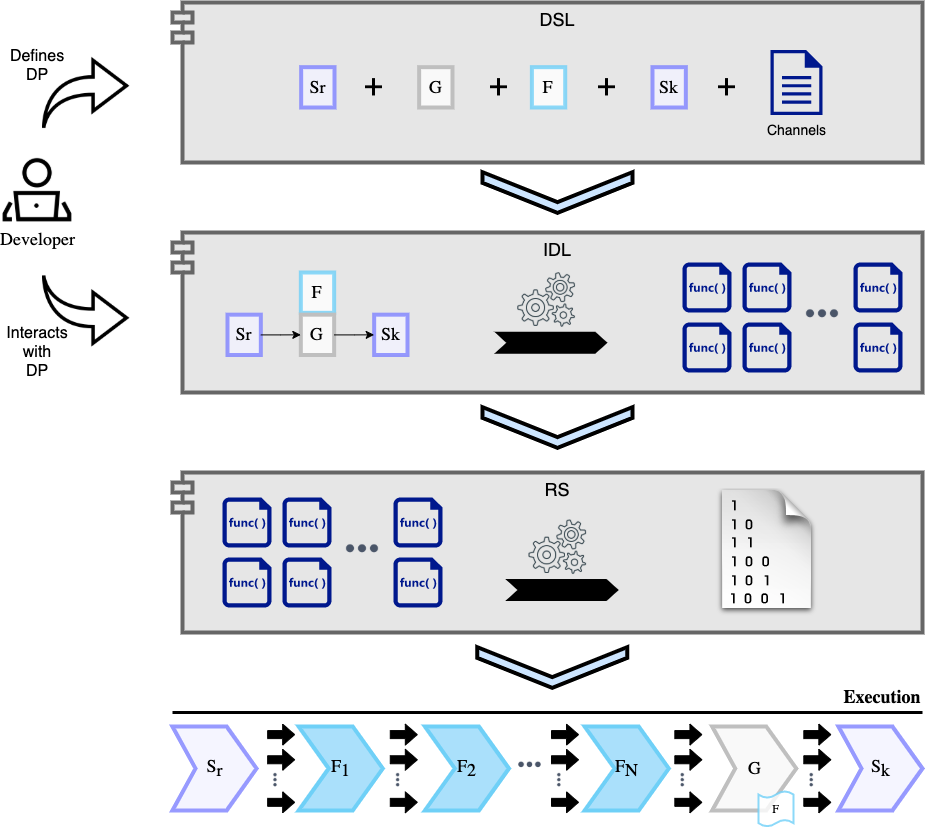
\includegraphics[width = 0.8\textwidth, height = 0.8\textheight]{dpf_haskell_v3}
  \end{center}
\end{frame}

  \begin{frame}[fragile]{DP Haskell Framework}
    \begin{center}
    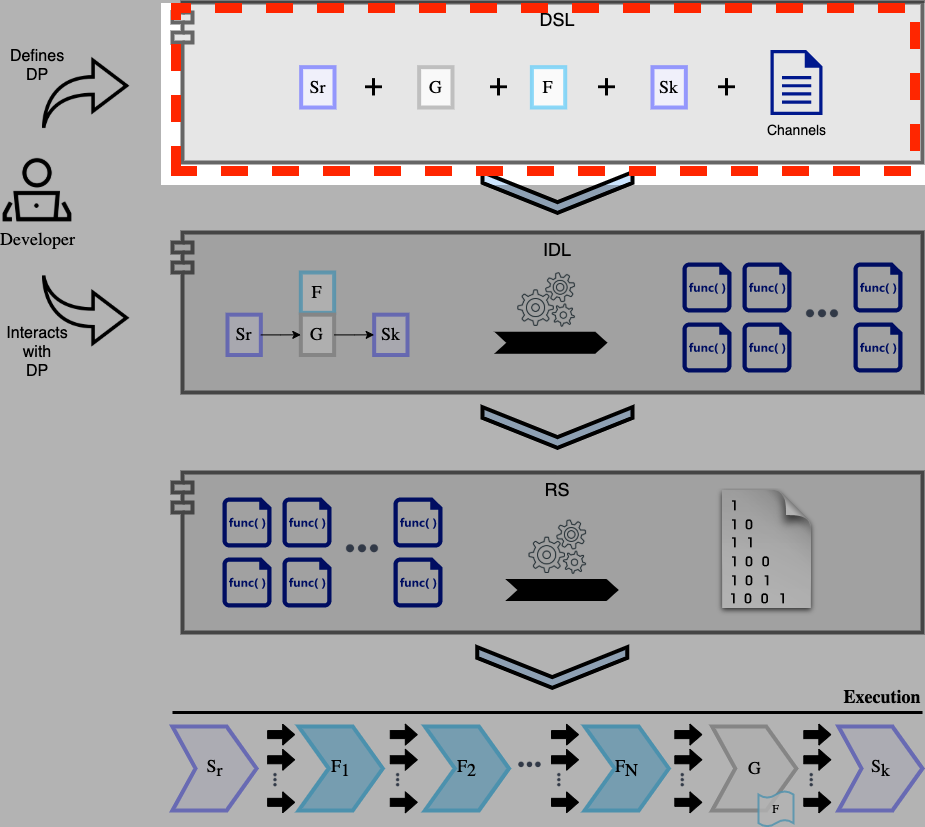
\includegraphics[width = 0.8\textwidth, height = 0.8\textheight]{dpf_haskell_v3-1}
  \end{center}
\end{frame}

\lstset{
  basicstyle=\itshape,
  literate={->}{$\rightarrow$}{2}
}

\begin{frame}[fragile]{DP Haskell Framework}
  \frametitle{DSL Grammar}
  \small
  \begin{equation*}
    \boxed{
     \begin{aligned}
    G_{dsl} = (N, \Sigma, DB, P)
    \end{aligned}
    }
\end{equation*}
\tiny
    \begin{equation*}
        \boxed{
         \begin{aligned}
        N &= \{DP,S_r,S_k,G,F_b,CH,CH_s\},\\
        \Sigma &= \{\text{\mintinline{haskell}{Source}},\text{\mintinline{haskell}{Generator}},\text{\mintinline{haskell}{Sink}},\text{\mintinline{haskell}{FeedbackChannel}},\text{\mintinline{haskell}{Type}},\text{\mintinline{haskell}{Eof}},\text{\mintinline{haskell}{:=>}},\text{\mintinline{haskell}{:<+>}}\},
        \end{aligned}
        }
    \end{equation*}
  \small
  \begin{equation*}
    \boxed{
      \begin{aligned}
    P = \{\\
    DP  &\rightarrow S_r\ \text{\mintinline{haskell}{:=>}}\ G\ \text{\mintinline{haskell}{:=>}}\ S_k\ |\ S_r\ \text{\mintinline{haskell}{:=>}}\ G\ \text{\mintinline{haskell}{:=>}}\ F_b\ \text{\mintinline{haskell}{:=>}}\ S_k,\\
    S_r &\rightarrow \text{\mintinline{haskell}{Source}}\ CH_s,\\
    G   &\rightarrow \text{\mintinline{haskell}{Generator}}\ CH_s,\\
    S_k &\rightarrow \text{\mintinline{haskell}{Sink}},\\
    F_b &\rightarrow \text{\mintinline{haskell}{FeedbackChannel}} CH,\\
    CH_s &\rightarrow \text{\mintinline{haskell}{Channel}}\ CH,\\
    CH &\rightarrow \text{\mintinline{haskell}{Type :<+>}}\ CH\ |\ \text{\mintinline{haskell}{Eof}}\}
  \end{aligned}
  }
  \end{equation*}
\end{frame}

\begin{frame}[fragile]{DP Haskell Framework}
  \begin{itemize}
    \item The specification of \textbf{DP} in the Language is compile time checked (\textit{Type-safe})
  \end{itemize}    
  \begin{exampleblock}{Type Level DSL}
    \begin{minted}[fontsize=\small,breaklines,highlightlines={7-17}]{shell}      
ghci> import DynamicPipeline
ghci> type DPExample = Source (Channel (Int :<+> Eof)) :=> Generator (Channel (Int :<+> Eof)) :=> Sink
type DPExample :: *
type DPExample =
Source (Channel (Int :<+> Eof))
:=> (Generator (Channel (Int :<+> Eof)) :=> Sink)
ghci> :t mkDP @DPExample
mkDP @DPExample
:: forall k (st :: k) filterState filterParam.
    Stage (WriteChannel Int -> DP st ())
    -> GeneratorStage DPExample filterState filterParam st
    -> Stage (ReadChannel Int -> DP st ())
    -> DP st ()    
  \end{minted}
  \end{exampleblock}
\end{frame}

\begin{frame}[fragile]{DP Haskell Framework}
  \begin{center}
    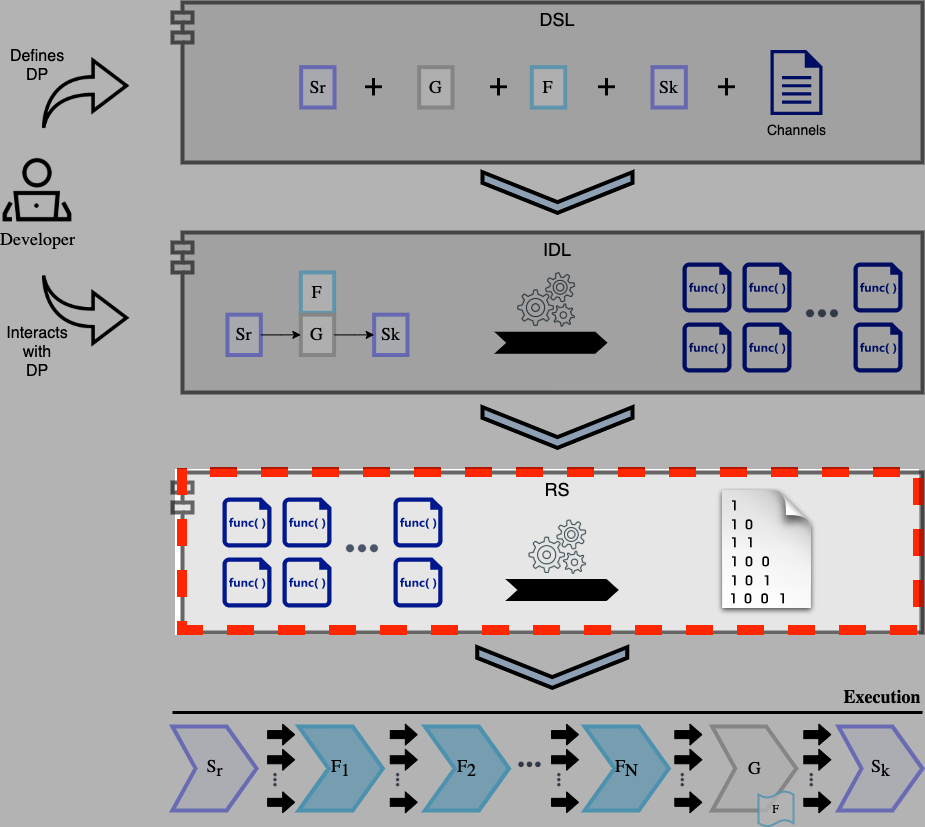
\includegraphics[width = 0.8\textwidth, height = 0.8\textheight]{dpf_haskell_v3-3}
  \end{center}
\end{frame}

\begin{frame}[fragile]{DP Haskell Framework}
  \begin{block}{Runtime System}
    \begin{itemize}
      \item \textbf{DP Monad}:
      \begin{itemize} 
      \item Monad with Existential Type to not escape DP Context. (\textit{Rank-2 Polymorphic type})
      \item Associativity Monad law guarantees execution flow (\mintinline{haskell}{ source >>= generator >>= sink }) 
      \end{itemize}
    \end{itemize}
  \end{block}
  \end{frame}

\begin{frame}[fragile]{DP Haskell Framework}
  \begin{block}{Runtime System}
    \begin{itemize}
      \item \textbf{DP Monad}:
      \begin{itemize} 
      \item Monad with Existential Type to not escape DP Context. (\textit{Rank-2 Polymorphic type})
      \item Associativity Monad law guarantees execution flow (\mintinline{haskell}{ source >>= generator >>= sink }) 
      \end{itemize}
      \item \textbf{Filter / Stage}: 
      \begin{itemize}
        \item Use of \mintinline{haskell}{unfold} to generate dynamic filter computations (\textit{Anamorphism})
        \item Use of \mintinline{haskell}{fold} to reduce results to Sink (\textit{Catamorphism})
      \end{itemize}
    \end{itemize}
  \end{block}
  \end{frame}

\begin{frame}[fragile]{DP Haskell Framework}
  \begin{block}{Runtime System}
    \begin{itemize}
      \item \textbf{DP Monad}:
      \begin{itemize} 
      \item Monad with Existential Type to not escape DP Context. (\textit{Rank-2 Polymorphic type})
      \item Associativity Monad law guarantees execution flow (\mintinline{haskell}{ source >>= generator >>= sink }) 
      \end{itemize}
      \item \textbf{Filter / Stage}: 
      \begin{itemize}
        \item Use of \mintinline{haskell}{unfold} to generate dynamic filter computations (\textit{Anamorphism})
        \item Use of \mintinline{haskell}{fold} to reduce results to Sink (\textit{Catamorphism})
      \end{itemize}
      \item \textbf{Multithreading}: \mintinline{shell}{async} library
    \end{itemize}
  \end{block}
  \end{frame}

\begin{frame}[fragile]{DP Haskell Framework}
\begin{block}{Runtime System}
  \begin{itemize}
    \item \textbf{DP Monad}:
    \begin{itemize} 
    \item Monad with Existential Type to not escape DP Context. (\textit{Rank-2 Polymorphic type})
    \item Associativity Monad law guarantees execution flow (\mintinline{haskell}{ source >>= generator >>= sink }) 
    \end{itemize}
  \item \textbf{Filter / Stage}: 
    \begin{itemize}
      \item Use of \mintinline{haskell}{unfold} to generate dynamic filter computations (\textit{Anamorphism})
      \item Use of \mintinline{haskell}{fold} to reduce results to Sink (\textit{Catamorphism})
    \end{itemize}
    \item \textbf{Multithreading}: \mintinline{shell}{async} library
    \item \textbf{Channels}: \mintinline{shell}{unagi-chan} library
  \end{itemize}
\end{block}
\end{frame}

\begin{frame}[fragile]{DP Haskell Framework}
  \begin{center}
    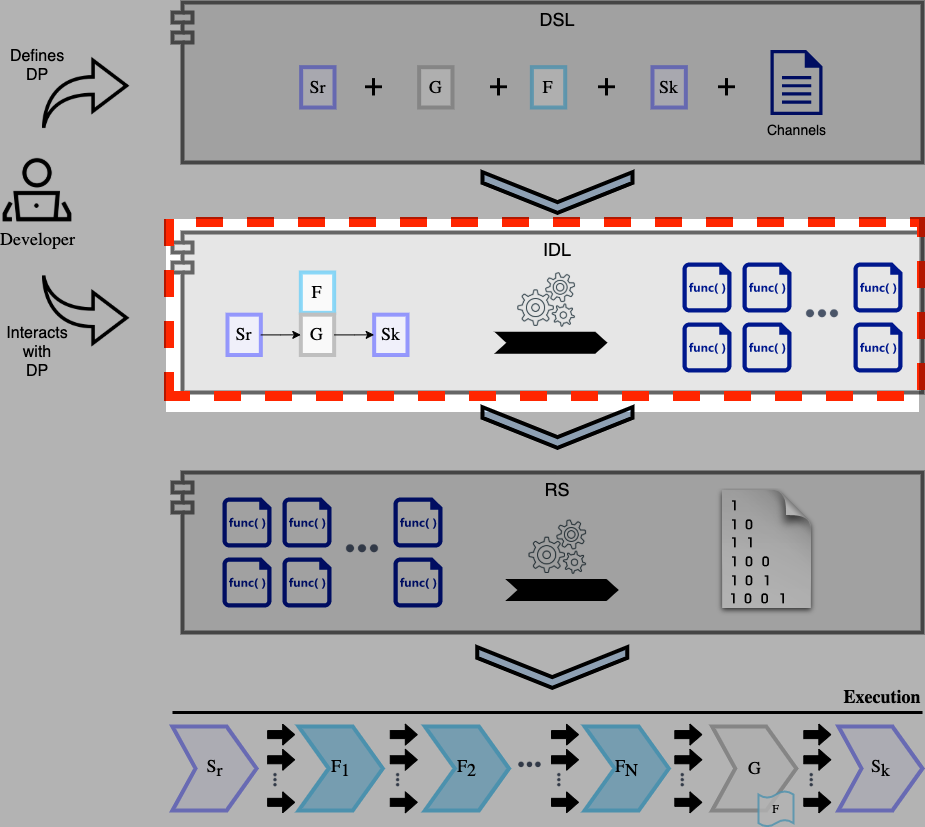
\includegraphics[width = 0.8\textwidth, height = 0.8\textheight]{dpf_haskell_v3-2}
  \end{center}
\end{frame}

\begin{frame}[fragile]{DP Haskell Framework}
  \begin{block}{IDL}
    \begin{minted}[fontsize=\small,breaklines]{shell}      
ghci> type DPExample = Source (Channel (Int :<+> Eof)) :=> Generator (Channel (Int :<+> Eof)) :=> Sink
type DPExample :: *
type DPExample =
Source (Channel (Int :<+> Eof))
:=> (Generator (Channel (Int :<+> Eof)) :=> Sink)
  \end{minted}
\end{block}
\end{frame}

\begin{frame}[fragile]{DP Haskell Framework}
  \begin{block}{IDL}
    \begin{minted}[fontsize=\small,breaklines,highlightlines={7-11}]{shell}      
ghci> type DPExample = Source (Channel (Int :<+> Eof)) :=> Generator (Channel (Int :<+> Eof)) :=> Sink
type DPExample :: *
type DPExample =
Source (Channel (Int :<+> Eof))
:=> (Generator (Channel (Int :<+> Eof)) :=> Sink)
      
ghci> :t withSource @DPExample
withSource @DPExample
:: forall k (st :: k).
    (WriteChannel Int -> DP st ())
    -> Stage (WriteChannel Int -> DP st ())
  \end{minted}
\end{block}
\end{frame}

\begin{frame}[fragile]{DP Haskell Framework}
  \begin{block}{IDL}
    \begin{minted}[fontsize=\small,breaklines,highlightlines={7-9}]{shell}      
ghci> :t withSource @DPExample
withSource @DPExample
:: forall k (st :: k).
    (WriteChannel Int -> DP st ())
    -> Stage (WriteChannel Int -> DP st ())
    
ghci> let source' = withSource @DPExample  $ \wc -> unfoldT ([1..10] <> [1..10]) wc identity
ghci> :t source'
source' :: forall k (st :: k). Stage (WriteChannel Int -> DP st ())
  \end{minted}
\end{block}
\end{frame}

\begin{frame}[fragile]{DP Haskell Framework}
  \begin{block}{IDL}
    \begin{minted}[fontsize=\small,breaklines,highlightlines={2-8}]{shell}      
ghci> :t withGenerator @DPExample
withGenerator @DPExample
:: forall k filter (st :: k).
    (filter -> ReadChannel Int -> WriteChannel Int -> DP st ())
    -> Stage
        (filter -> ReadChannel Int -> WriteChannel Int -> DP st ())    
  \end{minted}
\end{block}
\end{frame}

\begin{frame}[fragile]{DP Haskell Framework}
  \begin{block}{IDL}
    \begin{minted}[fontsize=\small,breaklines,highlightlines={2-8}]{shell}      
ghci> :t withGenerator @DPExample
withGenerator @DPExample
:: forall k filter (st :: k).
    (filter -> ReadChannel Int -> WriteChannel Int -> DP st ())
    -> Stage
        (filter -> ReadChannel Int -> WriteChannel Int -> DP st ())    
  \end{minted}
\end{block}
\begin{block}{Techniques}
  \begin{itemize}
    \item First Class Families
    \item Type-level Defunctionalization 
    \item Defunctionalization
    \item Associated Type Families
  \end{itemize}
\end{block}
\end{frame}

\begin{frame}[fragile]{DP Haskell Framework}
  \begin{block}{}
    Library released on Hackage \\
    https://hackage.haskell.org/package/dynamic-pipeline
    \begin{center}
      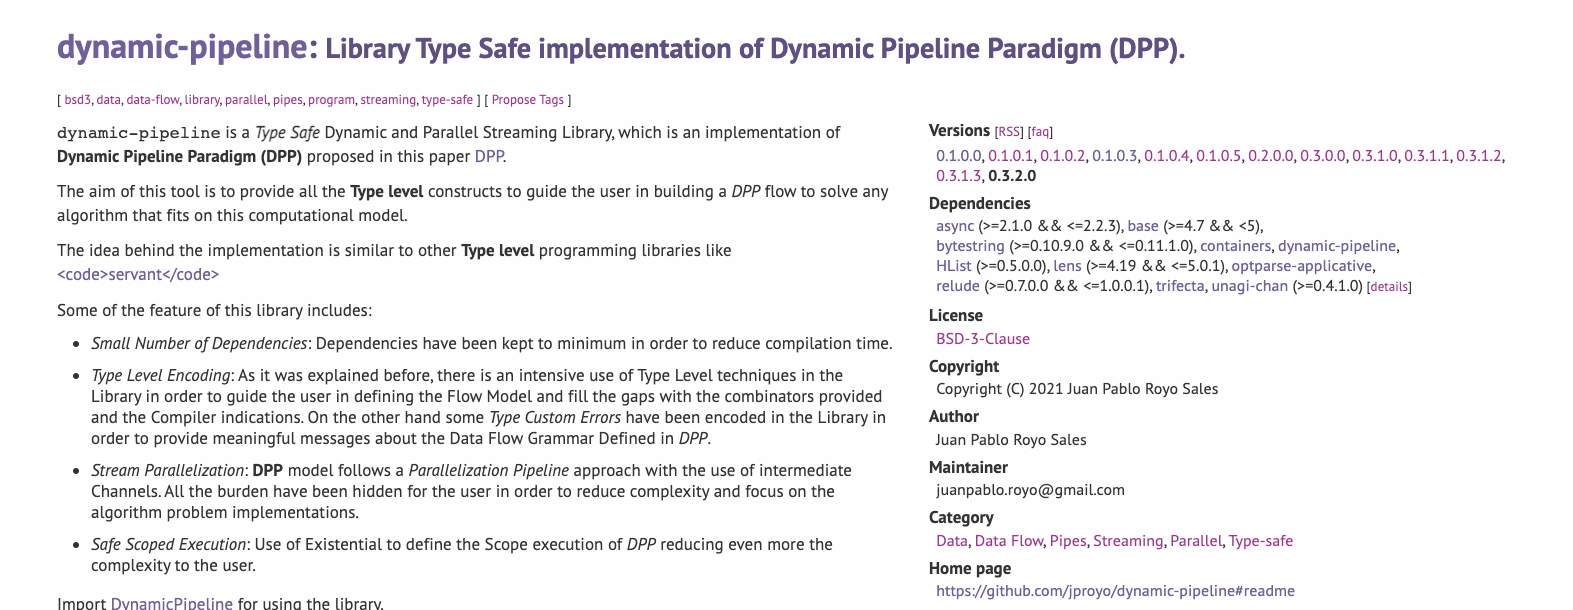
\includegraphics[width = 0.9\textwidth, height = 0.6\textheight]{dp-fw-hs}
    \end{center}  
  \end{block}
\end{frame}


  \subsection{Algorithm for Incrementally Enumerating BT in BG}
  \begin{frame}[fragile]{Algorithm for Incrementally Enumerating BT in BG (IEBT)}
  \begin{center}
  \large The algorithm consists in \textbf{2 (two) main phases} 
  \end{center}  
  \vspace{2em}   
  \begin{itemize}
    \setlength\itemsep{2em}
    \item \textbf{First Phase}: A \underline{\color{red}Graph Index} structure is created
  \end{itemize}
\end{frame}

\begin{frame}[fragile]{Algorithm for Incrementally Enumerating BT in BG (IEBT)}
  \begin{center}
  \large The algorithm consists in \textbf{2 (two) main phases} 
  \end{center}     
  \vspace{2em}   
  \begin{itemize}
    \setlength\itemsep{2em}
    \item {\color{light}\textbf{First Phase}: A Graph Index structure is created}
    \item \textbf{Second Phase}: Local \underline{\color{red}Queries} can be submitted to the index
  \end{itemize}
\end{frame}

\begin{frame}[fragile]{Algorithm for Incrementally Enumerating BT in BG (IEBT)}
  \begin{center}
  \large A \textbf{Bipartite Graph} is an undirected graph $G=(V,E)$  such that $V=(U\cup L)$, $U\cap L=\emptyset$ and $E\subseteq U\times L$.
  \end{center}     
  \begin{center}
    \small \emph{w.l.g.} $U \subseteq \mathbb{N}, L \subseteq \mathbb{N}$ and $(U, <)$, $(L, <)$ are \emph{strict total orders}
  \end{center}            
  \begin{figure}
    \centering
    \resizebox{0.7\textwidth}{!}{\inputtikz{bipartite}}
  \end{figure}
\end{frame}

\begin{frame}[fragile]{Algorithm for Incrementally Enumerating BT in BG (IEBT)}
  \begin{center}
  Let the triples $\mu=(u_1, u_2, u_3)$ and $\ell=(l_1, l_2,l_3)$ on $U$ and $L$, respectively, i.e.  $\{u_1, u_2, u_3\} \subseteq U$, $\{l_1, l_2,l_3\} \subseteq L$. 
  The 6-cycle $(u_1,l_1,u_2,l_3,u_3,l_2,u_1)$  is a \textbf{Bitriangle} in $G$. 
  \end{center}      
  \begin{figure}
    \centering
    \resizebox{0.7\textwidth}{!}{\inputtikz{bitriangle}}
  \end{figure}
\end{frame}

\begin{frame}[fragile]{IEBT: First Phase - Graph Index Structures}
  \begin{center}
    \large We \textbf{introduce} a conceptual framework based on abstract \textbf{compacted structures} to specify the algorithm.
  \end{center}    
  \begin{table}[H]
    \centering
    \resizebox{0.8\textwidth}{!}{
    \begin{tabular}{c c}
     \begin{tabular}{c}\underline{\color{red}Aggregated Wedges}\\$\la l, W_l \ra$\end{tabular} & \begin{tabular}{l}\resizebox{5cm}{2cm}{\inputtikz{bipartite_awg_a}\inputtikz{bipartite_awg_c}}\end{tabular}\\
    \end{tabular}
    }
   \end{table}
\end{frame}

\begin{frame}[fragile]{IEBT: First Phase - Graph Index Structures}
  \begin{center}
    \large We \textbf{introduce} a conceptual framework based on abstract \textbf{compacted structures} to specify the algorithm.
  \end{center}    
  \begin{table}[H]
    \centering
    \resizebox{0.8\textwidth}{!}{
    \begin{tabular}{c c}
     \begin{tabular}{c}\underline{\color{red}Aggregated Wedges}\\$\la l, W_l \ra$\end{tabular} & \begin{tabular}{l}\resizebox{5cm}{2cm}{\inputtikz{bipartite_awg_a}\inputtikz{bipartite_awg_c}}\end{tabular}\\
     \begin{tabular}{c}\underline{\color{red}Aggregated Double Wedges} \\$\la (l_1, l_2), U_l \ra$\end{tabular} & \begin{tabular}{l}\resizebox{4cm}{2cm}{\inputtikz{bipartite_adwg_a}}\end{tabular}\\
    \end{tabular}
    }
   \end{table}
\end{frame}

\begin{frame}[fragile]{IEBT: First Phase - Graph Index Structures}
  \begin{center}
    \large We \textbf{introduce} a conceptual framework based on abstract \textbf{compacted structures} to specify the algorithm.
  \end{center}    
  \begin{table}[H]
    \centering
    \resizebox{0.8\textwidth}{!}{
    \begin{tabular}{c c}
     \begin{tabular}{c}\underline{\color{red}Aggregated Wedges}\\$\la l, W_l \ra$\end{tabular} & \begin{tabular}{l}\resizebox{5cm}{2cm}{\inputtikz{bipartite_awg_a}\inputtikz{bipartite_awg_c}}\end{tabular}\\
     \begin{tabular}{c}\underline{\color{red}Aggregated Double Wedges} \\$\la (l_1, l_2), U_l \ra$\end{tabular} & \begin{tabular}{l}\resizebox{4cm}{2cm}{\inputtikz{bipartite_adwg_a}}\end{tabular}\\
     \begin{tabular}{c}\underline{\color{red}Aggregated Bitriangles} \\$\langle \ell, \hat{U}_l\rangle$\end{tabular} & \begin{tabular}{l}\resizebox{4cm}{2cm}{\inputtikz{bipartite_abt_a}}\end{tabular}\\
    \end{tabular}
    }
   \end{table}
\end{frame}

\begin{frame}[fragile]{IEBT: Second Phase - Queries}
  \begin{center}
    \large We \textbf{define} a \underline{\color{red}Query Operator} for extracting bitriangles from the index which can be:
  \end{center}  
  \vspace{2em}
  \begin{itemize}
    \setlength\itemsep{2em}
    \item \textbf{$\mathcal{P}(U+L)$}: For extracting BT \underline{\color{blue}according to vertices} from $U$ or $L$
  \end{itemize}  
\end{frame}

\begin{frame}[fragile]{IEBT: Second Phase - Queries}
  \begin{center}
    \large We \textbf{define} a \underline{\color{red}Query Operator} for extracting bitriangles from the index which can be:
  \end{center}  
  \vspace{2em}
  \begin{itemize}
    \setlength\itemsep{2em}
    \item \textbf{$\mathcal{P}(U+L)$}: For extracting BT \underline{\color{blue}according to vertices} from $U$ or $L$
    \item \textbf{$\mathcal{P}(E)$}: For extracting BT \underline{\color{blue}according to edges} from $E$
  \end{itemize}  
\end{frame}

% \begin{frame}[fragile]{Algorithm for Incrementally Enumerating BT in BG}
%   \begin{center}
%     We build first \textbf{Aggregated Wedges}: a pair $\la l, W_l \ra$, where $l \in L$, $W_l \subseteq U$ and for all $u \in W_l$, the edge  $(u,l)\in E$
%   \end{center}    
%   \begin{figure}
%     \centering
%     \resizebox{0.8\textwidth}{!}{\inputtikz{bipartite_awg_a}\inputtikz{bipartite_awg_b}\inputtikz{bipartite_awg_c}}
%   \end{figure}
% \end{frame}

% \begin{frame}[fragile]{Algorithm for Incrementally Enumerating BT in BG}
%   \begin{center}
%     Then, \textbf{Aggregated Double Wedges}: a pair  $\la (l_1, l_2), U_l \ra$, where $\{l_1,l_2\}\subseteq L$ and  for all $u_i \in I, u_j \in J$ and $u_k \in K$, $\{(u_i, l_1), (u_j, l_1), (u_j, l_2), (u_k, l_2)\} \in E$.
%     $I \subseteq U, J \subseteq U$ and $K \subseteq U$, where $I, J$ and $K$ are disjoint sets. 
%   \end{center}    
%   \begin{figure}
%     \centering
%     \resizebox{0.6\textwidth}{!}{\inputtikz{bipartite_adwg_a}}
%   \end{figure}
% \end{frame}

% \begin{frame}[fragile]{Algorithm for Incrementally Enumerating BT in BG}
%   \begin{center}
%     \textbf{Finally}, \textbf{Aggregated Bitriangles}: is a pair  $\langle \ell, \hat{U}_l\rangle$, 
%     where $\ell=(l_1, l_2, l_3)$ is a triple on $L$, $l_1 < l_2 < l_3$ and for all $\la I, J, K\ra$ and for all $\mu=(u_i, u_j, u_k)$ such that $u_i \in I, u_j \in J, u_k \in K$, $BT_{\ell}^{\mu} \in \mathsf{BT}$.
%   \end{center}    
%   \begin{figure}
%     \centering
%     \resizebox{0.6\textwidth}{!}{\inputtikz{bipartite_abt_a}}
%   \end{figure}
% \end{frame}


\begin{frame}[fragile]{Algorithm for Incrementally Enumerating BT in BG}
  \begin{center}
    \textbf{Dynamic Pipeline} Configuration for Enumerating BT in BG
  \end{center}    
  \begin{figure}
    \centering  
    \resizebox{0.7\textwidth}{!}{\inputtikz{btDP}}
  \end{figure}
  \begin{figure}
    \centering  
    \resizebox{0.7\textwidth}{!}{\inputtikz{btDP_actor1}}
  \end{figure}
\end{frame}

% \begin{frame}[fragile]{Algorithm for Incrementally Enumerating BT in BG}
%   \begin{center}
%     \large Lets see how the Actors' Filter solve this
%   \end{center} 
%   \begin{center}
%   \resizebox{1\textwidth}{!}{  
%   \begin{algorithm}[H]
%     \SetKwInOut{P}{Filter Parameter}
%     \SetKwInOut{FS}{Filter State}
%     \SetKwInOut{IC}{Input Channels}
%     \SetKwInOut{OC}{Output Channels}
%     \SetKwFunction{actora}{actor1}
%     \SetKwFunction{actorb}{actor2}
%     \SetKwFunction{actorc}{actor3}
%     \SetKwFunction{actord}{actor4}
%     \SetKwFunction{filter}{filter}
%     \SetKwProg{df}{def}{:}{end}
%     \SetAlgorithmName{}{fil}{}
%     \SetAlgoRefName{[A4]}
%     \P{$l \in L$}
%     \FS{$\st = \aw + \mathcal{P}(\dw) + \mathcal{P}(\at)$}
%     \IC{$ IC = \la IC_E, IC_{W_l1}, IC_{W_l2}, IC_Q, IC_{BT} \ra $}
%     \OC{$ OC = \la OC_E, OC_{W_l1}, OC_{W_l2}, OC_Q, OC_{BT} \ra $}
%     \df{\filter{}}{
%           $\actora()$\\
%           $\actorb()$\\
%           $\actorc()$\\
%           $\actord()$\\
%     }
%   \end{algorithm}  
%   }  
% \end{center} 
% \end{frame}

\begin{frame}[fragile]{Algorithm for Incrementally Enumerating BT in BG}
  \begin{center}
    \underline{\textbf{\texttt{actor1}: Aggregated Wedges}}
  \end{center}
  \begin{tikzpicture}[overlay, remember picture]
    \node[xshift=-4cm,yshift=-5cm] at (current page.north east) {
      \resizebox{5cm}{2cm}{\inputtikz{bipartite_awg_a}\inputtikz{bipartite_awg_c}}
    };
  \end{tikzpicture}
  \resizebox{!}{0.3\textheight}{  
    \begin{algorithm}[H]
      \SetKwFunction{acta}{actor1}
      \SetKwProg{df}{def}{:}{end}
      \df{\acta{}}{
      $\la l, W_l \ra \leftarrow \gs$\\
      \ForAll{$(u',l') \in IC_E$}
      {%
      \color{red!80}
      \uIf{$l = l'$}{
        $W_l \leftarrow W_l \cup \{u'\}$
      }\Else{$\p((u',l'),OC_E)$}
      }
      \If{$|W_l| > 1$}{
          \color{red!80}
          $\us(\la l, W_l \ra)$\\ 
          $\p(\la l, W_l \ra, OC_{W_l1})$\\
      }
      }
      \end{algorithm}
  }
\end{frame}

\begin{frame}[fragile]{Algorithm for Incrementally Enumerating BT in BG}
  \begin{center}
    \underline{\textbf{\texttt{actor2}: Aggregated Double Wedges}}
  \end{center}
  \begin{tikzpicture}[overlay, remember picture]
    \node[xshift=-4cm,yshift=-5cm] at (current page.north east) {
      \resizebox{5cm}{3cm}{\inputtikz{bipartite_adwg_a}}
    };
  \end{tikzpicture}
  \resizebox{!}{0.4\textheight}{  
    \begin{algorithm}[H]
      \SetKwFunction{actb}{actor2}
      \SetKwProg{df}{def}{:}{end}
      \BlankLine
      \df{\actb{}}{
      $\la l, W_l \ra \leftarrow \gs$\\
      \ForAll{$\la l', W_l' \ra \in IC_{W_l1}$}{
        \color{red!80}
        $\p(\la l', W_l \ra, OC_{W_l1})$\\
        \color{black}
        $\dwi \leftarrow \emptyset$\\
        \If{$W_l' \cap W_l \neq \emptyset$}{ 
              \color{blue!80}
              $(l_l, l_u) \leftarrow (\argmin_{l,l'}, \argmax_{l,l'})$\\
              \uIf{$l < l'$}{
                    $(W_{l_l}, W_{l_u}) \leftarrow (W_l, W_l')$
              }\Else{
                    $(W_{l_l}, W_{l_u}) \leftarrow (W_l', W_l)$
              }
              $I \leftarrow W_{l_l} \setminus W_{l_u}$\\ 
              $J \leftarrow W_{l_l} \cap W_{l_u}$\\
              $K \leftarrow W_{l_u} \setminus W_{l_l}$\\
              $U_l \leftarrow \la I, J, K\ra$\\
              \color{red!80}
              $\dwi \leftarrow dw \cup \{\la (l_l, l_u), U_l \ra\}$
        }
      }
      \color{red!80}$\us(\dwi)$
      }
      \end{algorithm}
  }  
\end{frame}

\begin{frame}[fragile]{Algorithm for Incrementally Enumerating BT in BG}
  \begin{center}
    \underline{\textbf{\texttt{actor3}: Aggregated Bitriangles}}
  \end{center}
  \begin{tikzpicture}[overlay, remember picture]
    \node[xshift=-3.5cm,yshift=-6.5cm] at (current page.north east) {
      \resizebox{5cm}{3cm}{\inputtikz{bipartite_abt_a}}
    };
  \end{tikzpicture}
  \resizebox{!}{0.4\textheight}{  
    \begin{algorithm}[H]
      \SetKwFunction{actc}{actor3}
      \SetKwProg{df}{def}{:}{end}
      \BlankLine
      \df{\actc{}}{
        $\dwi \leftarrow \gs$\\
        $\ati \leftarrow \emptyset$\\
        \ForAll{$\la l', W_l \ra \in IC_{W_l2}$}{
          \color{red!80}
          $\p(\la l', W_l \ra, OC_{W_l2})$\\ 
          \ForEach{$\la (l_l, l_u), \la I, J, K \ra \ra \in \dwi, l_l < l' \land l_u > l'$}{
            \color{blue!80}
            $I' \leftarrow I \cup J$\\
            $K' \leftarrow K \cup J$\\
            \If{$W_l \cap I' \neq \emptyset \land W_l \cap K' \neq \emptyset$}{
                  $I' \leftarrow I' \cap W_l$\\
                  $K' \leftarrow K' \cap W_l$\\
                  $\hat{U}_l  \leftarrow \la I', J, K' \ra$\\
                  \color{red!80}
                  $\ati \leftarrow \ati \cup \big\{\la (l_l, l', l_u), \hat{U}_l \ra\big\}$
                  \color{black}
            }
          }
        }      
        \color{red!80}
        $\us(\ati)$\\
      }
    \end{algorithm}
  }  
\end{frame}

\begin{frame}[fragile]{Algorithm for Incrementally Enumerating BT in BG}
  \begin{center}
    \underline{\textbf{\texttt{actor4}: Process Query to incrementally enumerate Bitriangles}}
  \end{center}
  \begin{tikzpicture}[overlay, remember picture, show background rectangle]
    \node[xshift=-3cm,yshift=-5.5cm,label=above:{If $\mathcal{P}(U+L) = \{3\}$ then},label=below:{will be enumerated}] at (current page.north east) {
      \resizebox{3cm}{2cm}{\inputtikz{bipartite_bt_a}}
    };
  \end{tikzpicture}
  \resizebox{!}{0.4\textheight}{  
    \begin{algorithm}[H]
      \SetKwFunction{butV}{buildBtVertex}
      \SetKwFunction{butE}{buildBtEdge}      
      \SetKwFunction{actd}{actor4}
      \SetKwProg{df}{def}{:}{end}
      \BlankLine
      \df{\actd{}}{
        $\ati \leftarrow \gs$\\
        \ForAll{$Q \in IC_Q$}{
          \ForEach{$\la (l_l, l_m, l_u), \la I,J,K \ra \ra \in \ati$}{
            \color{blue!80}
            \Switch{$Q$}{
                  \color{red!80}
                  \Case{$\mathcal{P}(U + L)$}{
                    \color{blue!80}
                    \If{$\mathcal{P}(U + L) \cap \{l_l, l_m, l_u\} \neq \emptyset \lor \mathcal{P}(U + L) \cap (I \cup J \cup K) \neq \emptyset$}{
                      \color{red!80}
                      $\btii \leftarrow \butV(\la (l_l, l_m, l_u), \la I,J,K \ra \ra), \mathcal{P}(U + L))$\\
                      \ForAll{$\bti \in \btii$}{
                        $\p(\bti, OC_{BT})$
                      }
                      \color{black}
                    }
                  }
                  \color{blue!80}
                  \Case{$\mathcal{P}(E)$}{
                      \tcp*[h]{SAME FOR EDGES......}\\
                  }
            }
          }
        }
      }
    \end{algorithm}
  }  
\end{frame}


\begin{frame}[fragile]{Algorithm for Incrementally Enumerating BT in BG}
  \begin{block}{Correctness of the Algorithm}
    We need to prove that the algorithm \textbf{can enumerate all bitriangles} in the graph and also that there are \textbf{no duplicates in the enumeration}.
  \end{block}
\end{frame}


\begin{frame}[fragile]{Algorithm for Incrementally Enumerating BT in BG}
  \begin{theorem}[Uniqueness] 
    Given a bipartite graph $G = ((U\cup L),E)$, $\forall \btii\in\bt$  \acrshort{iebt} stores $\btii$ in an $\ati\in \at$ only once.
  \end{theorem}
  \vspace{1.5cm}
  \begin{theorem}[All Bitriangles can be enumerated]
    Given a bipartite graph $G$, if the bitriangle $\btii = (u_1,l_1,u_2,l_3,$ $u_3,l_2,u_1)\in \bt$, then $\btii$  can be enumerated.
  \end{theorem}  
\end{frame} 

\iffalse
\begin{frame}[fragile]{Algorithm for Incrementally Enumerating BT in BG}
  \begin{proof}[Proof. No Bitriangles are duplicated]   
  Let $\bti =$  $(u_1,l_1,u_2,l_3,u_3,l_2,u_1)$, such that $l_1 < l_2 <l_3$. For every feasible permutation  starting with a node in $U$ we are going to proof that only one will be accepted by $\ab$, or $\ac$.  
  \begin{itemize}
        \item According to lines 7-12 of $\ab$ $(u_1,l_2,u_3,l_3,u_2,l_1,u_1)$ is  not accepted  when constructing elements of $\dw$ to be used by $\ac$  because $l_2 > l_1$ 
        \item According to lines 7 of $\ac$ $(u_3,l_2,u_1,l_1,u_2,l_3,u_3)$ is not accepted because $l_2 > l_1$
        \item According to lines 7-12 of $\ab$ $(u_3,l_3,u_2,l_1,u_1,l_2,u_3)$ is  not accepted  when constructing elements of $\dw$ to be used by $\ac$  because  $l_3 > l_2$
        \item According to lines 7-12 of $\ab$ $(u_2,l_3,u_3,l_2,u_1,l_1,u_2)$ not accepted because $l_3 > l_1 $
  \end{itemize}
  \end{proof}  
\end{frame}

\begin{frame}[fragile]{Algorithm for Incrementally Enumerating BT in BG}
  \begin{proof}[Proof. (Cont.) No Bitriangles are duplicated]   
  Let $\bti =$  $(u_1,l_1,u_2,l_3,u_3,l_2,u_1)$, such that $l_1 < l_2 <l_3$. For every feasible permutation  starting with a node in $U$ we are going to proof that only one will be accepted by $\ab$, or $\ac$.  
  \begin{itemize}
        \item According to lines 7-12 of $\ab$ and line 7 in $\ac$ $(u_2,l_1,u_1,l_2,u_3,l_3,u_2)$ is accepted because $l_1 < l_3 $ and $l_1 < l_2 <l_3$ 
        \item According to  line 7 in $\ac$ $(u_1, l_1,u_2,l_3,u_3,l_2,u_1)$ is not accepted because $l_3 > l_2$
  \end{itemize}
  Therefore the  only bitriangle  constructed by the algorithm is the one that satisfies $l_1 < l_2 < l_3$ where $u_1,u_2,u_3$  are distinct and $u_1$ is incident to $l_1$ and $l_2$, $u_2$ is incident to $l_1$ and $l_3$ and $u_3$ is incident to $l_2$ and $u_3$.
  \end{proof}  
\end{frame}


\begin{frame}[fragile]{Algorithm for Incrementally Enumerating BT in BG}
  \begin{proof}[All Bitriangles can be enumerated] 
    \begin{itemize}
      \item Let $\bti =$  $(u_1,l_1,u_2,l_3,u_3,l_2,u_1)$, such that $l_1 < l_2 <l_3$ is present in the graph. 
      \item When $\aaa$ acting in filter $F_{l_1}$ ends reading all the edges, $\{u_1,u_2\} \subseteq W_{l_1}$. Also when $\aaa$ in filter $F_{l_3}$ ends reading all the edges, $\{u_2,u_3\} \subseteq W_{l_3}$. 
      \item As $l_1 < l_3$ in $\ab$, in lines 7-12, in filter $F_{l_1}$ or in filter $F_{l_3}$, the pair $(l_1,l_3)$  will be added to $\mathsf{dw}$.
      \item When $\ac$ in lines 7-16, in filter $F_{l_1}$ or in filter $F_{l_3}$ receives $(l_2, W_{l_2})$  will construct the corresponding  $BT$ because of the condition in line 10 is satisfied (non empty intersection). 
    \end{itemize}    
    Therefore, the bitriangle is stored in $\mathsf{bt}$ an thus $(u_1,l_1,u_2,l_3,u_3,l_2,u_1)$ can be listed by $\ad$.
  \end{proof}
  
\end{frame} 
\fi


  \begin{frame}{Agenda}
    \section{Empirical Evaluation}
    \tableofcontents[currentsection,hideothersubsections]
  \end{frame}

  \begin{frame}[fragile]{Research Questions}
    \begin{itemize}
      \setlength\itemsep{2em}
        \item Does \acrshort{dpbt} generate \textbf{incremental results} regardless of the size of the graph?
        \item Does the type of query \textbf{$Q$ impact} on the execution of \acrshort{dpbt}?
        \item How effectively \acrshort{dpbt} implements a \textbf{\emph{pay-as-you-go} model}?
        \item Does \acrshort{dpbt} handle \textbf{memory and threads} efficiently?
    \end{itemize}        
\end{frame}

\begin{frame}[fragile]{Experiments}
    \begin{itemize}
      \setlength\itemsep{2em}
      \item \textbf{Continuous behavior Analysis}: using \acrshort{dt} and \acrshort{dk} to assess the continuous behavior capabilities.
      \item \textbf{Benchmark Analysis}: to identify how the behavior of \acrshort{dpbt} varies depending on the type of query command.
      \item \textbf{Performance Analysis} \acrfull{ghc} Profiling for one of the graphs to measure multithreading and memory allocation. 
    \end{itemize}
\end{frame}

\begin{frame}[fragile]{Experiment Configuration}
  \begin{block}{Datasets Tested}
    \begin{table}[H]
      \centering
      \resizebox{1\textwidth}{!}{
      \begin{tabular}{|p{0.25\linewidth}|c|c|c|c|c|}
        \hline
       \textbf{Network} & \textbf{$|U|$} & \textbf{$|L|$} & \textbf{$|E|$} & \textbf{Wedges} & \textbf{\#\acrshort{bt}} \\
       \hline
       \rowcolor{yellow!35}
       Dbpedia & 18422 & 168338 & 233286 & $1.45 \times 10^8$ & \color{red}\bf$3.62 \times 10^8$\\
       \hline
       Moreno Crime & 829 & 551 & 1476 & 4816 & 211\\
       \hline
       \rowcolor{yellow!35}
       Opsahl UC Forum  & 899 & 522 & 33720 & 174069 & \color{red}\bf$2.2 \times 10^7$ \\
       \hline
       Wang Amazon & 26112 & 799 & 29062 & $3.4 \times 10^6$ & 110269\\
       \hline
      \end{tabular}
      }
     \end{table}
  \end{block}
  \begin{block}{Hardware Environment}
    \begin{itemize}
          \item \emph{HPC Cluster at UPC}
          \item $x86$ $64$ bits
          \item $24$-Core Intel(R) Xeon(R) CPU X5650 processor of $2.67$ GHz
          \item \emph{Hyper-threading} enable
          \item $40 GB$ up to $120 GB$ of RAM for the biggest \acrfull{dbpedia} graph
      \end{itemize}        
  \end{block}
\end{frame}

\begin{frame}[fragile]{Experiment Configuration}
  \begin{block}{Test Case Scenarios}
    \begin{table}[H]
      \centering
      \resizebox{1\textwidth}{!}{
        \begin{tabular}{|l|c|c|}
          \hline
          \textbf{Scenario ID} & \textbf{Name} & \textbf{Search by}\\
          \hline
          E-H & Edge High & edge with high incidence \\
          \hline
          E-L & Edge Low & edge with low incidence \\
          \hline
          E-M & Edge Medium & edge with medium incidence \\
          \hline
          VL-H & $l \in L$ High & vertex in lower layer with high incidence \\
          \hline
          VL-L & $l \in L$ Low & vertex in lower layer with low incidence \\
          \hline
          VL-M & $l \in L$ Medium & vertex in lower layer with medium incidence \\
          \hline
          VU-H & $u \in U$ High & vertex in upper layer with high incidence \\
          \hline
          VU-L & $u \in U$ Low & vertex in upper layer with low incidence \\
          \hline
          VU-M & $u \in U$ Medium & vertex in upper layer with medium incidence \\
          \hline
        \end{tabular}
    }
     \end{table}
  \end{block}
\end{frame}

\begin{frame}[fragile]{E1: Continuous Behavior: \acrshort{dt} and \acrshort{dk}}
  \begin{table}[H]
    \centering
    \resizebox{1\textwidth}{!}{
    \begin{tabular}{|p{0.25\linewidth}|c|c|c|}
      \hline
     \textbf{Network} & \textbf{Scenario ID} & \textbf{\acrshort{dt} Metric}  & \textbf{\acrshort{dk} Metric}\\
     \hline
     \multirow{3}{*}{Moreno Crime}
      & VU-H & $6.05 \times 10^2$ & $0.00$\\
      & VL-H & $7.95 \times 10^3$ & $0.00$\\
      & E-H & $9.85 \times 10^3$ & $0.00$\\
      \hline
      \multirow{3}{*}{Dbpedia}
      & VU-H & $3.32 \times 10^{13}$ & $1.97 \times 10^5$\\
      & VL-H &  $1.81 \times 10^{14}$ & $2.34 \times 10^4$\\
      & E-H &  $1.75 \times 10^{13}$ & $3.28 \times 10^5$\\
      \hline
      \multirow{3}{*}{Opsahl UC Forum}
      & VU-H &  $1.99 \times 10^{12}$ & $1.27 \times 10^5$\\
      & VL-H &  $6.44 \times 10^{11}$ & $1.90 \times 10^5$\\
      & E-H &  $1.02 \times 10^{11}$ & $2.93 \times 10^5$\\
      \hline
      \multirow{3}{*}{Wang Amazon}
      & VU-H & $1.50 \times 10^7$ & $43.6$\\
      & VL-H & $2.24 \times 10^7$ & $63.1$\\
      & E-H & $8.06 \times 10^6$  & $42.3$\\
      \hline
    \end{tabular}
    }
   \end{table}
\end{frame}

\begin{frame}[fragile]{E1: Continuous Behavior: \acrshort{dt} and \acrshort{dk}}
  \begin{figure}[!htp]
    \centering
    \begin{subfigure}[t]{0.45\textwidth}
     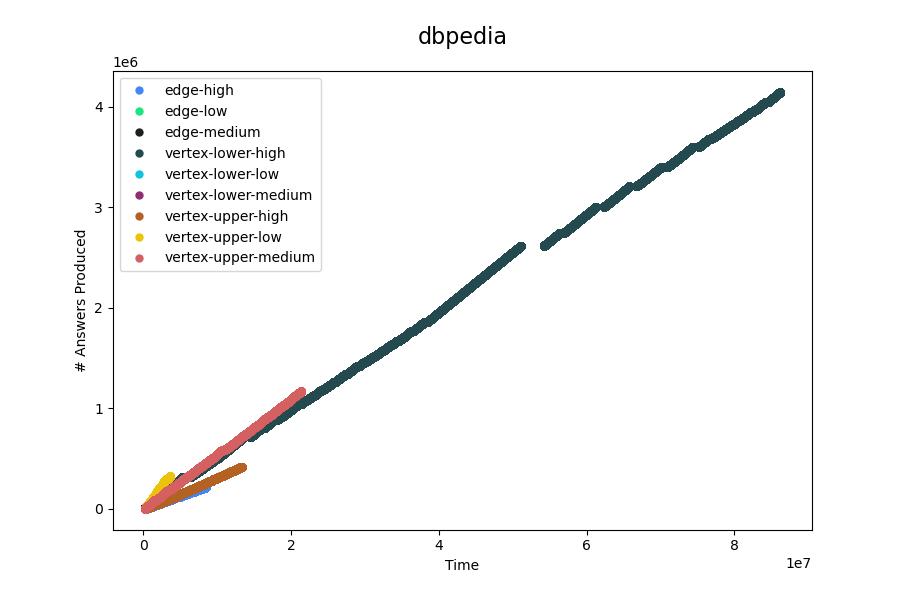
\includegraphics[width=1\linewidth, height=0.4\textheight]{experiments/diepfy/dbpedia.png}
    \end{subfigure}\hfill
    \begin{subfigure}[t]{0.45\textwidth}
     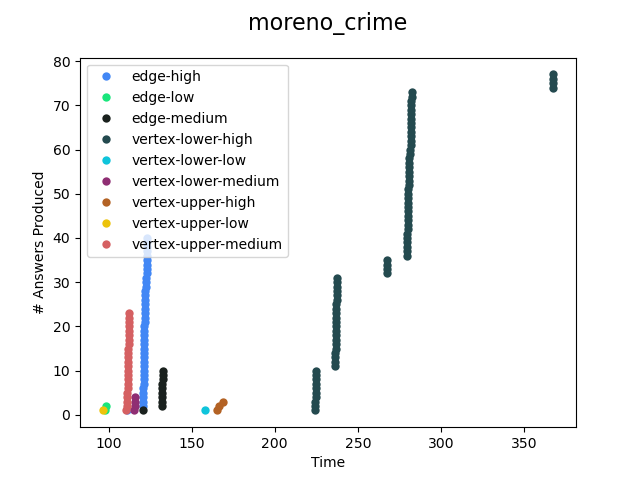
\includegraphics[width=1\linewidth, height=0.4\textheight]{experiments/diepfy/moreno_crime.png}
    \end{subfigure}
    \vspace{0.5cm}
  
    \begin{subfigure}[t]{0.45\textwidth}
     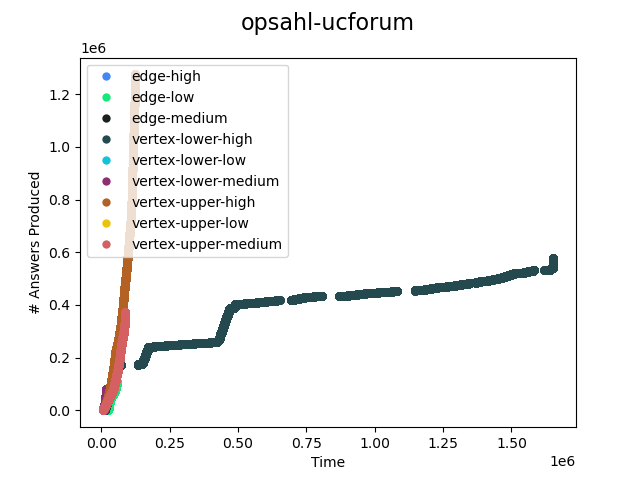
\includegraphics[width=1\linewidth, height=0.4\textheight]{experiments/diepfy/opsahl-ucforum.png}
    \end{subfigure}\hfill
    \begin{subfigure}[t]{0.45\textwidth}
      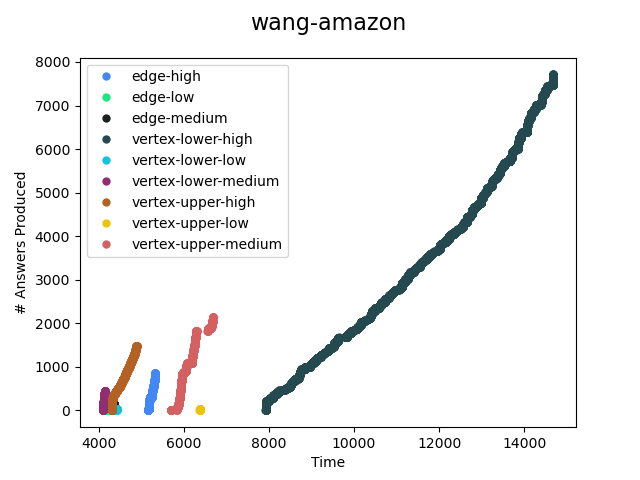
\includegraphics[width=1\linewidth, height=0.4\textheight]{experiments/diepfy/wang-amazon.png}
     \end{subfigure}
   \end{figure}
  \end{frame}

\begin{frame}[fragile]{E2: Average Excution Time}
  \begin{table}[H]
    \centering
    \resizebox{1\textwidth}{0.4\textheight}{%
    \begin{tabular}{|c|c|c|c|}
    \hline
     \textbf{Network} & \textbf{Scenario ID}  & \textbf{Average Execution Time} & \textbf{Standard deviation}\\
     \hline
     \multirow{6}{*}{Moreno Crime} & VL-L & $656$ ms & $13.0$ ms \\
     & VL-M & $669$ ms & $18.7$ ms \\ 
     & VL-H & $723$ ms & $72.2$ ms \\ 
     & E-L & $694$ ms & $4.7$ ms \\ 
     & E-M & $655$ ms & $14.9$ ms \\ 
     & E-H & $655$ ms & $21.1$ ms \\ 
     \hline
     \multirow{6}{*}{Opsahl UC Forum} & VL-L & $5.6$ s & $940$ ms \\
     & VL-M & $18.1$ s & $5.03$ s \\ 
     & VL-H & $70.8$ s & $2.03$ s \\ 
     & E-L & $41.9$ s & $2.87$ s \\ 
     & E-M & $26.7$ s & $5.63$ s \\ 
     & E-H & $26.2$ s & $4.05$ s \\
    \hline
    \multirow{6}{*}{Wang Amazon} & VL-L & $6.5$ s & $1.05$ s \\
    & VL-M & $5.91$ s & $994$ ms \\ 
    & VL-H & $10.2$ s & $2.66$ s \\ 
    & E-L & $6.4$ s & $1.08$ s \\ 
    & E-M & $5.71$ s & $863$ ms \\ 
    & E-H & $5.91$ s & $1.04$ s \\
   \hline
   \end{tabular}
    }
  \end{table}
  \end{frame}

  \iffalse
  \begin{frame}[fragile]{E2: Average Excution Time}
  \begin{figure}[H]
    \begin{center}
      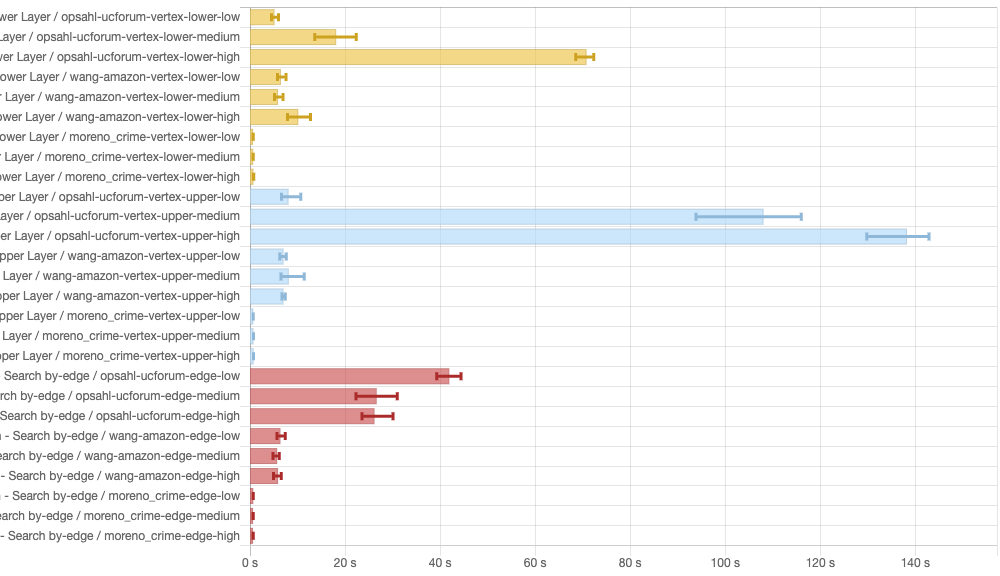
\includegraphics[width=1\textwidth]{experiments/bench_1}
    \end{center}
  \end{figure}
  \end{frame}
  \fi

\begin{frame}[fragile]{E2: Total Excution Time}
  \begin{figure}[H]
    \begin{center}
       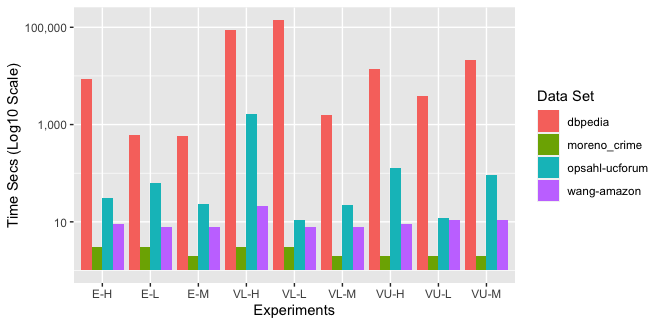
\includegraphics[width=1\textwidth] {experiments/execution_time_by_experiments}
    \end{center}
  \end{figure}
\end{frame}

\begin{frame}[fragile]{E3: Performance Analysis - Multithreading}
    \begin{figure}[!htp]
      \centering
      \begin{subfigure}[t]{0.45\textwidth}
        \begin{center}
          \textbf{General Overview}
        \end{center}
        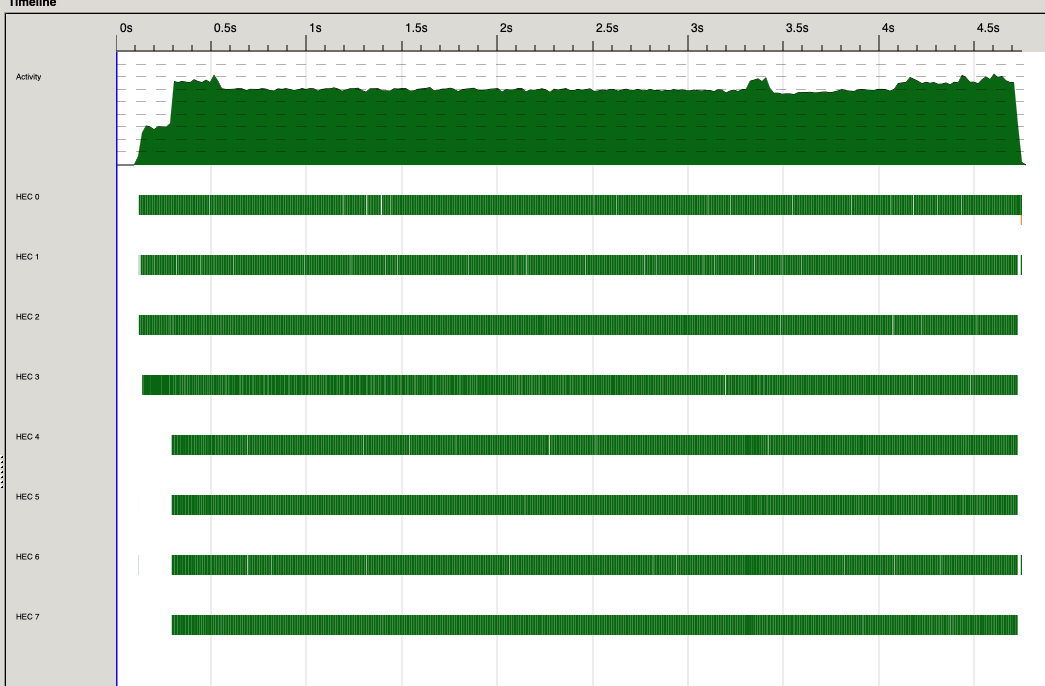
\includegraphics[width=1\linewidth, height=0.7\textheight]{experiments/thread/general_overview.png}
      \end{subfigure}\hfill
      \begin{subfigure}[t]{0.45\textwidth}
        \begin{center}
          \textbf{Middle Execution Time}
        \end{center}
        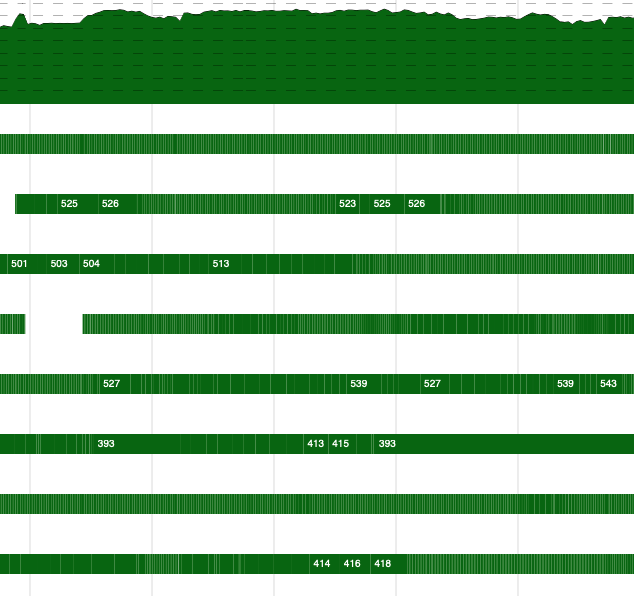
\includegraphics[width=1\linewidth, height=0.7\textheight]{experiments/thread/middle.png}
      \end{subfigure}
    \end{figure}
  \end{frame}


\begin{frame}[fragile]{E3: Performance Analysis - Memory Allocation}
  \begin{figure}[H]
    \begin{center}
      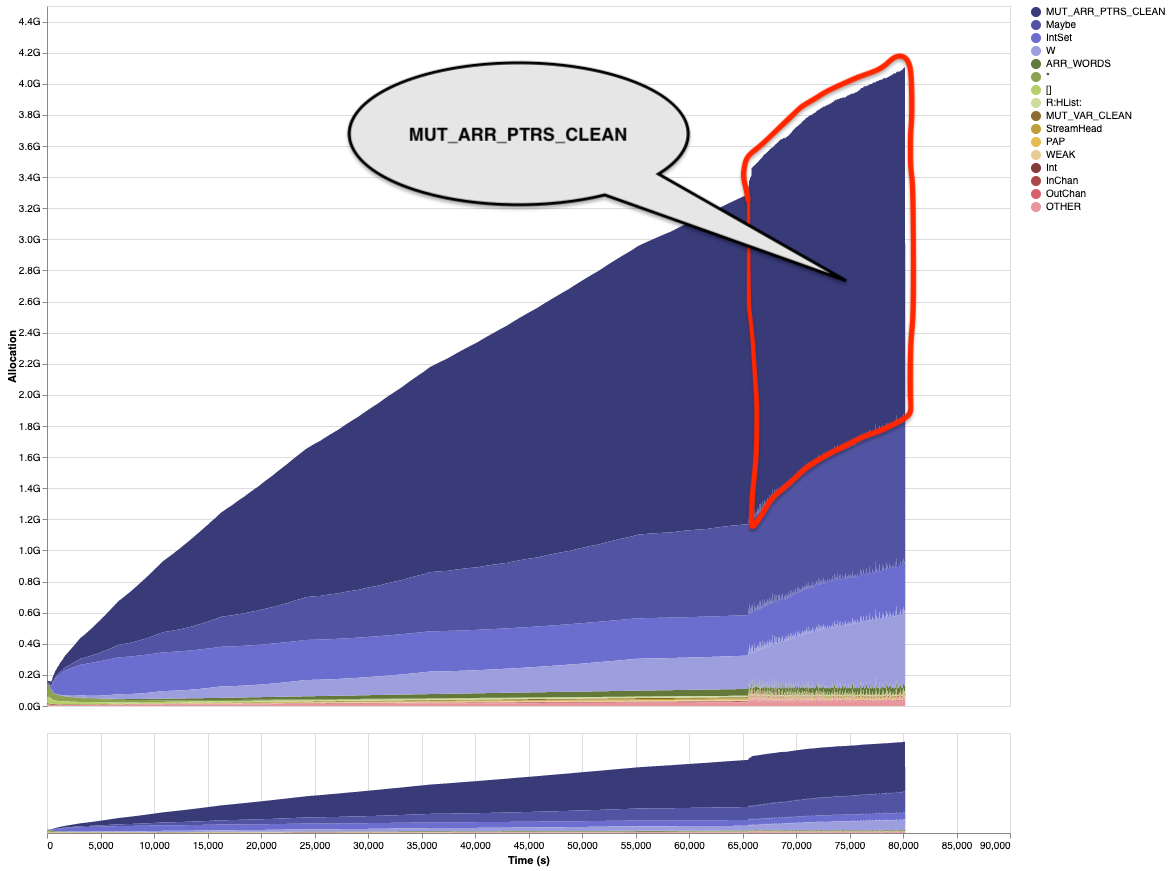
\includegraphics[width=0.8\textwidth] {experiments/mem/overview_1}
    \end{center}
  \end{figure}
\end{frame}

\begin{frame}[fragile]{Empirical Evaluation: Conclusions}
  \begin{itemize}
    \setlength\itemsep{1.5em}
    \item Results of \textbf{dief$@$t} and \textbf{dief$@$k} metrics indicates continuous behavior.
    \item \textbf{High values} of \textbf{\emph{Average Running Time}} and \textbf{\emph{Total Running Time}} are suggesting an effective implementation of a \emph{pay-as-you-go} model of \acrshort{dpbt}.
    \item Results in \texttt{ThreadScope} tool indicates an \textbf{efficient use of the parallel model}.
    \item Results in \texttt{eventlog2html} tool indicates \textbf{efficient memory consumption}.
  \end{itemize} 
\end{frame}


  \begin{frame}
    \begin{figure}
      \centering
      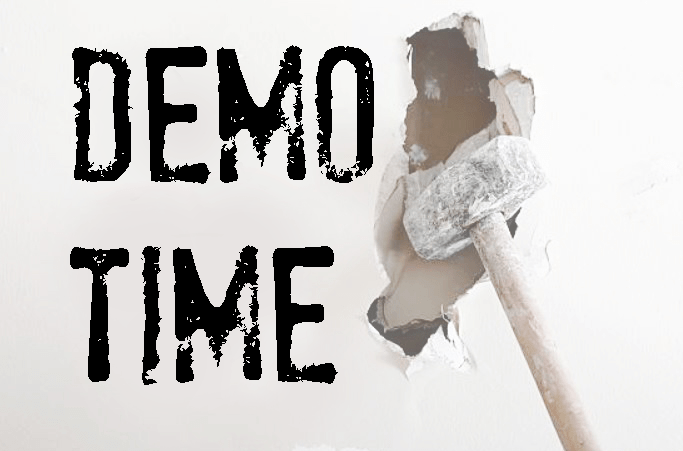
\includegraphics[height=7.5cm]{demo-time}
    \end{figure}
  \end{frame} 

  \begin{frame}{Agenda}
    \section{Conclusions and Future Work}
    \tableofcontents[currentsection,hideothersubsections]
  \end{frame}

  \begin{frame}[fragile]{Conclusions and Future Work}
  \begin{block}{Conclusions}      
    \begin{itemize}
      \item \textbf{Robustness and Suitability} of the DP-Haskell 
    \end{itemize}
  \end{block}
\end{frame}

\begin{frame}[fragile]{Conclusions and Future Work}
  \begin{block}{Conclusions}      

  \begin{itemize}
    \item \textbf{Robustness and Suitability} of the DP-Haskell 
    \item \textbf{Ability to generate Incremental results} has been shown by $\mathtt{dief@t}$ metrics 
  \end{itemize}
\end{block}
\end{frame}

\begin{frame}[fragile]{Conclusions and Future Work}
  \begin{block}{Conclusions}      

  \begin{itemize}
    \item \textbf{Robustness and Suitability} of the DP-Haskell 
    \item \textbf{Ability to generate Incremental results} has been shown by $\mathtt{dief@t}$ metrics
    \item \textbf{Satisfactory Performance results} with an adequate Memory allocation and Execution times. 
  \end{itemize}
\end{block}
\end{frame}

\begin{frame}[fragile]{Conclusions and Future Work}
  \begin{block}{Future work}      
  \begin{itemize}
    \item \textbf{Explore other Algorithms} to be implemented with this Paradigm.\footnote{We are currently working on Bi-partite Graphs algorithms}
    \item \textbf{Improve DP Framework} implementing more combinators and abstractions to allow the user write better and faster programs.
  \end{itemize}
\end{block}
\end{frame}


  \begin{frame}[allowframebreaks]
    \frametitle{References}
    \bibliographystyle{amsalpha}
    \bibliography{Report.bib}
  \end{frame}

  \begin{frame}
    \begin{figure}
      \centering
      
\includegraphics[height=7.5cm]{thanks-question}
    \end{figure}
  \end{frame}  

  \iffalse
  \chapter{Appendix}
\section{Source Code}
All the source code of this research project can be found in \url{https://github.com/jproyo/upc-miri-tfm}, and it is publicly available for download.
In that source code there are three folders:

\begin{itemize}
  \item \textbf{connected-comp}: This contains the \acrshort{hs} source code done for the \autoref{prole} contribution related to \acrfull{wcc} using \acrshort{dp}.
  \item \textbf{bt-graph-dp}: This contains the \acrshort{hs} source code done for the specific problem of this work which is incremental enumeration of \acrlong{bt} in \acrlong{bg}.
  \item \textbf{doc}: Contains this document in LaTex format as well as \acrshort{prole21} presentation and paper.
\end{itemize}

\section{Running Experiments}\label{apx:running:experiments}
All the scripts and data for running the experiments are under \mintinline{shell}{bt-graph-dp/experiments} folder.
It is important to mention that we are not including in the source code distribution the networks themselves because you can search them on Konect~\cite{konect} by the reference in this work.
We are going to describe how to run the different experiments exposed on \autoref{experiments}. 

\paragraph{E1} In this case we have different experiments setups and we are going to describe how to run one case only.
For example for running the experiment setup $E-H$ on \acrshort{dbpedia} graph, assuming that you download the graph and call the file as 
\mintinline{shell}{input.txt} and it is inside of folder \mintinline{shell}{bt-graph-dp/experiments/diepfy/dbpedia}.
\begin{minted}[breaklines]{bash}
>>> cd bt-graph-dp
>>> stack build
>>> stack exec bt-graph-dp -- +RTS -A1G -H1G -N6 -c -RTS -f ./experiments/diepfy/dbpedia/input.txt -c ./experiments/diepfy/dbpedia/c-edge-high.txt -e dbpedia
\end{minted}


\paragraph{E2} In the case of benchmark analysis it is simple the following command
\begin{minted}{bash}
  >>> cd bt-graph-dp
  >>> stack build
  >>> stack exec benchmark
  \end{minted}

\setlength{\rightskip}{0pt plus 1 fil}
This is going to left the results in HTML file format under \mintinline{bash}{benchmark}.


\paragraph{E3} In the case of Memory and Thead Measurement you need to enable profiling flags.

For Memory
\begin{minted}[breaklines]{bash}
>>> cd bt-graph-dp
>>> stack build --profile
>>> stack exec bt-graph-dp -- +RTS -A10G -H10G -c -N12 -hy -l-agu -RTS -f ./experiments/diepfy/moreno_crime/input.txt -c ./experiments/diepfy/moreno_crime/c-edge-high.txt -e moreno_crime
\end{minted}

For ThreadScope
\begin{minted}[breaklines]{bash}
>>> cd bt-graph-dp
>>> stack build --profile
>>> stack exec bt-graph-dp -- +RTS -A10G -H10G -c -N12 -l -s -RTS -f ./experiments/diepfy/moreno_crime/input.txt -c ./experiments/diepfy/moreno_crime/c-edge-high.txt -e moreno_crime
\end{minted}

  \fi

  \end{document}